
\mysection{Division du travail}
Le travail a été divisé en plusieurs parties a fin de faciliter l'acquisition des résultats.

\mysubsection{Première Partie}
Ce partie consistait de lire l'article de WAN Yidong \cite{yidong} et des extraits de la thèse de Marjorie  Cosson \cite{cosson:tel-01374469}, pour comprendre le problème et ses implications. Autres lectures supplémentaire ont été faites, \cite{farina2015model} et \cite{mariani2013controllo}.

\mysubsection{Deuxième Partie}
Après la lecture des documents commençait l'étude et pris en main du logiciel DIgSILENT PowerFactory, en lisant et regardant les tutoriels a l'internet, en faisant quelques petits exemples du logiciel a fin d'apprendre les outils nécessaires pour faire les tests proposés et après la montage de la modèle du réseaux dans le PowerFactory, le diagramme montré dans la figure \ref{fig:Diagramme_du_reseaux} 

\mysubsection{Troisième Partie}
Pendant ce partie diverses scripts ont été crées en utilisant les langages MATLAB et Python:
\begin{itemize}
\item Pour charger les valeurs de puissance des charges.
\item Pour charger les valeurs de puissance des générateurs.
\item Pour calculer les gains entre les bus et les générateurs.
\item Pour faire des matrices de gains.
\item Pour créer des événements de charges et générateurs, faire des simulations et prendre les résultats en graphiques.
\end{itemize}

\mysubsection{Quatrième Partie}
Pendant la quatrième partie la interface entre le PowerFactory et MATLAB a été requise a fin de créer une modèle de régulateur au simulink et utiliser dans le PowerFactory. Le Régulateur a été déjà crée et quelques configurations dans le PowerFactory sont manquantes.


\mysubsection{Cinquième Partie}
La cinquième partie est la élaboration des rapports.



\begin{figure}[H]
	\begin{center}	
		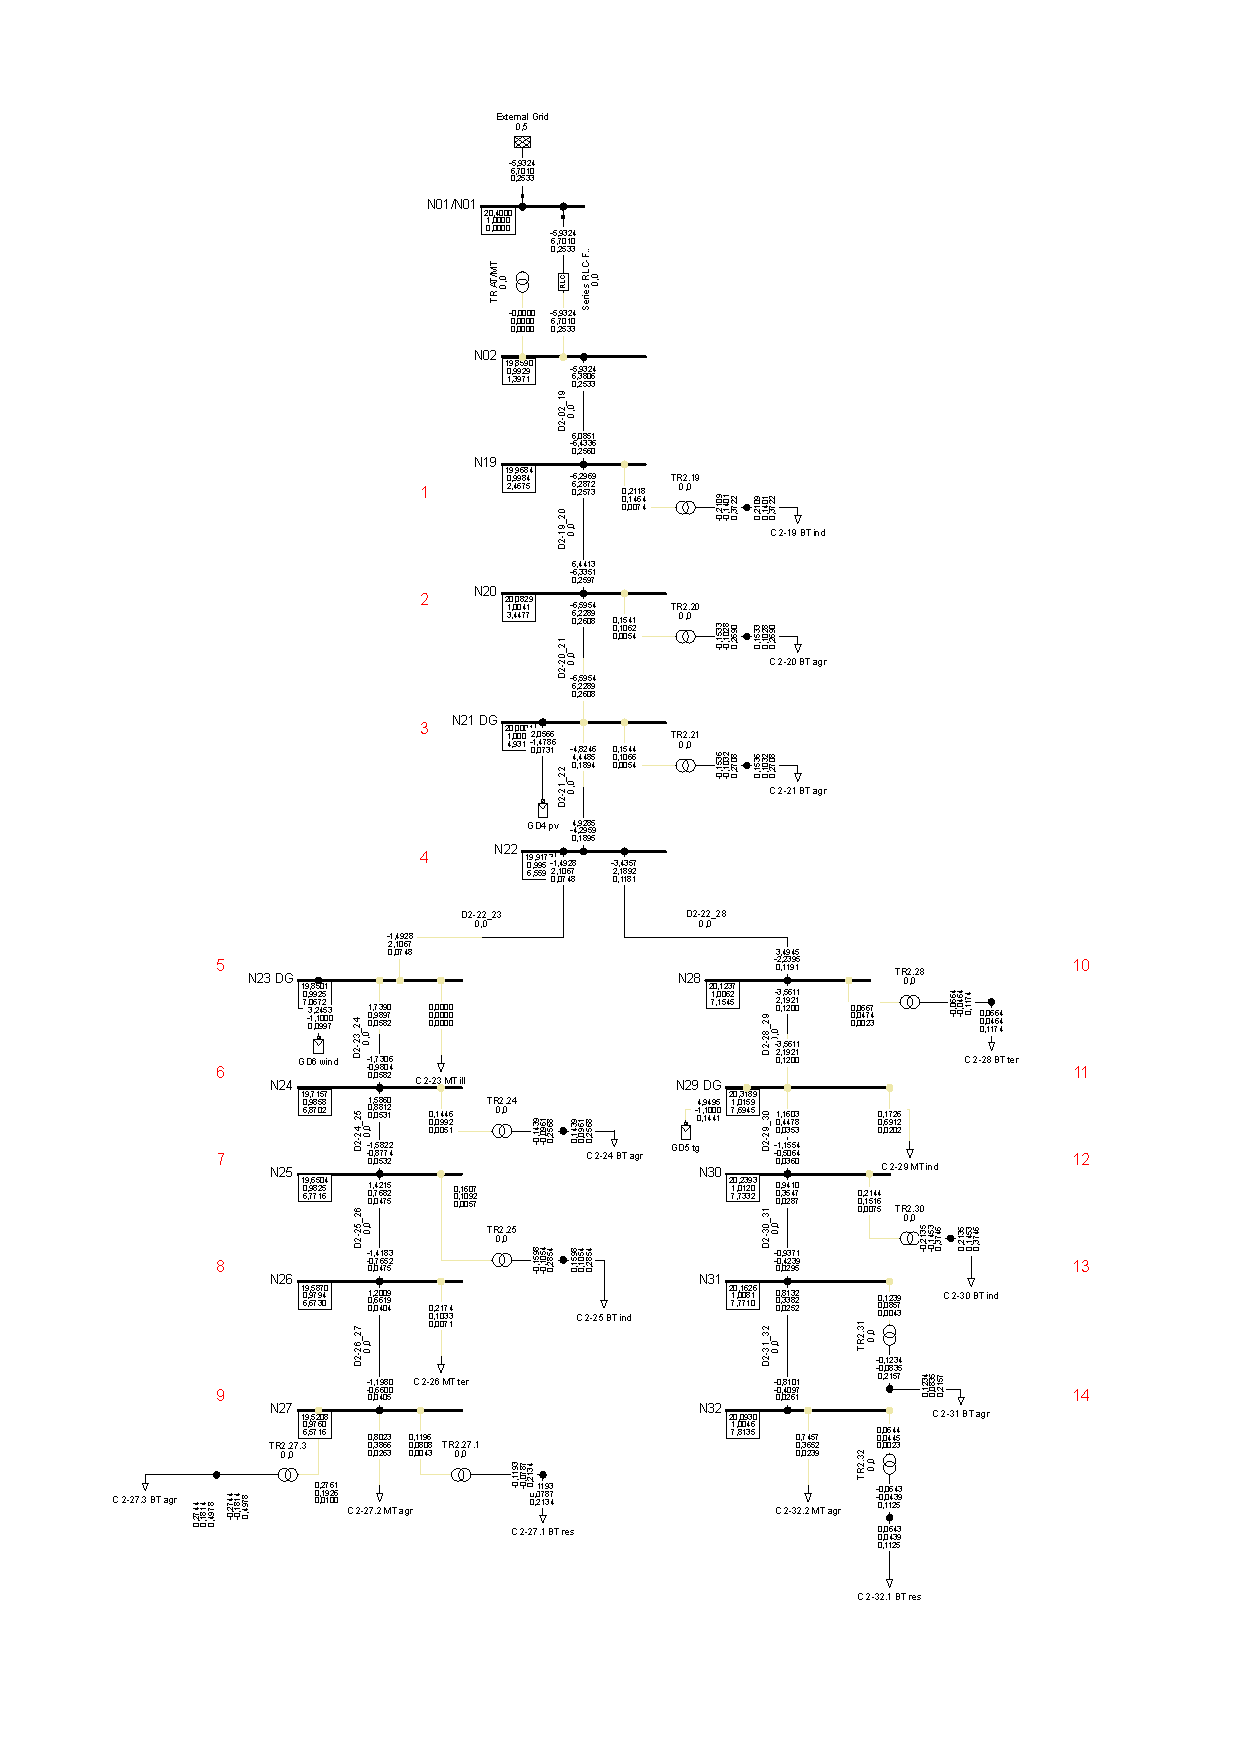
\includegraphics[width=\textwidth]{Division_du_travail/Diagramme_du_reseaux.pdf}
		\caption{Diagramme du reseaux}
		\label{fig:Diagramme_du_reseaux}
	\end{center}
\end{figure}
\pagebreak